\begin{appendices}
\pagestyle{plain}
% \begin{center}
% \chapter*{\centering Appendices}
% \addcontentsline{toc}{section}{Appendices}
% \end{center}
\newpage
\pagenumbering{roman}
\renewcommand{\thesubsection}{\Alph{subsection}}

%%%%%%%%%%%%%%%%%%%%%%%
% MODEL M0 DERIVATION %
%%%%%%%%%%%%%%%%%%%%%%%
\subsection{Model M$_0$ derivation} \label{appendix:M0.derivation}

Knowing seronegative individuals become seropositive at rate $\lambda_t$ and seropositive individuals revert at rate $\rho_t$, the proportion of seropositive individuals in a cohort $P$ is defined by the differential equation \cite{yman2016antibody}
%
\begin{equation}
    \frac{dP}{dt}=\lambda_t (1-P) - \rho_t P\ .
\end{equation}
%
\noindent
Considering model M$_0$, with constant transmission rates, $\lambda_t=\lambda$ and $\rho_t=\rho$, this equation can be solved to estimate the proportion of individuals of age $t$ at each cross-section.
%
\begin{equation}
\label{eq:apendix.2}
\begin{split}
    \int \frac{1}{\lambda(1-P)-\rho P}\ dP =& \int dt \Leftrightarrow \\
    \Leftrightarrow \int \frac{1}{\lambda-P(\lambda+\rho)}\ dP =&  \int dt \Leftrightarrow \\
    \Leftrightarrow -\frac{1}{\lambda+\rho} \int \frac{-(\lambda+\rho)}{\lambda-P(\lambda+\rho)}\ dP =&  \int dt \Leftrightarrow \\
    \Leftrightarrow -\frac{1}{\lambda+\rho} \ln(\lambda-P(\lambda+\rho)) =&\  t+c \Leftrightarrow \\
    \Leftrightarrow \  \ln(\lambda-P(\lambda+\rho)) =& -(\lambda+\rho)(t+c) \Leftrightarrow \\
    %\Leftrightarrow \  P(\lambda+\rho) =& \ \lambda - e^{ \left\{ -(\lambda+\rho)t-(\lambda+\rho)c\right\}} \Leftrightarrow \\
    \Leftrightarrow \  P =&\  \frac{\lambda - e^{ \left\{ -(\lambda+\rho)t-(\lambda+\rho)c\right\}}}{\lambda+\rho}\ .
\end{split}
\end{equation}

\noindent
Since a true seropositive state could only be achieved by being exposed to the malaria parasites (not accounting for the maternal acquired antibodies), this model assumes that no individual is seropositive at the moment of birth, i.e. $P(0)=0$, thus
%
\begin{equation}
\begin{split}
    \frac{\lambda - e^{ \left\{-(\lambda+\rho)0-(\lambda+\rho)c\right\}}}{\lambda+\rho} = &\  0 \Leftrightarrow \\
    \frac{\lambda - e^{ \left\{-(\lambda+\rho)c\right\}}}{\lambda+\rho} = &\  0 \Leftrightarrow \\
    %\Leftrightarrow \frac{e^{ \left\{-(\lambda+\rho)c\right\}}}{\lambda+\rho} = &\  \frac{\lambda}{\lambda+\rho} \Leftrightarrow \\
    \Leftrightarrow e^{ \left\{-(\lambda+\rho)c\right\}} =& \ \lambda \Leftrightarrow \\
    %\Leftrightarrow -(\lambda+\rho)c =& \ \ln(\lambda) \Leftrightarrow \\
    \Leftrightarrow c =& -\frac{\ln(\lambda)}{\lambda+\rho}\ ,
\end{split}
\end{equation}
%
\noindent
that can be directly applied onto previous equation (\ref{eq:apendix.2}),
%
\begin{equation}
\begin{split}
    %P =&\  \frac{\lambda - e^{ \left\{ -(\lambda+\rho)t+(\lambda+\rho)\frac{\ln(\lambda)}{\lambda+\rho}\right\}}}{\lambda+\rho} \\
    P =&\  \frac{\lambda - e^{ \left\{ -(\lambda+\rho)t+\ln(\lambda)\right\}}}{\lambda+\rho} \\
    =&\ \frac{\lambda-e^{\left\{ -(\lambda+\rho)t \right\}}\lambda}{\lambda+\rho} \\
    =& \frac{\lambda}{\lambda+\rho}\left(1- e^{\left\{ -(\lambda+\rho)t \right\}}\right)\ .
\end{split}
\end{equation}

\newpage



\subsection{Relationship between SCR, EIR, and the cutoff for SRR reducion}\label{appendix:EIR.and.SCR}

\begin{table}[H]
\centering
\caption[Relationship between SCR, EIR, and the cutoff for SRR reducion]{Relationship between SCR and the age in years at which SRR is expected to reduce from $\rho_1$ to $\rho_2$ (with $\rho_1 \geq \rho_2$). As previously described, estimates for SCR have a somewhat direct translation to the entomological inoculation rate measure (EIR), that identifies the number of infective bites received per person in a year, in a human population.}
\label{tab:EIR.to.SCR}
\begin{tabular}{ccc}
\toprule
EIR & SCR, $\lambda$ & \begin{tabular}[c]{@{}c@{}}Age of SRR\\reduction, $\hat{\uptau}$\end{tabular}      \\ 
\midrule
100  & 0.2900 & 3, 5                                                                  \\
10   & 0.0969 & 5, 10                                                                 \\
1    & 0.0324 & 5, 10                                                                 \\
0.1  & 0.0108 & 10, 15, 20                                                            \\
0.01 & 0.0036 & 10, 15, 20                                                            \\
\bottomrule
\end{tabular}
\end{table}


%%%%%%%%%%%%%%%%%%
% M11 VERSUS M12 %
%%%%%%%%%%%%%%%%%%
\subsection{M$_{1,2}$ \textit{vs.} M$_{1,1}$} \label{appendix:M12vM11}

%%%%% MSP1 %%%%%
\begin{sidewaystable}
\centering
\caption[Likelihood ratio test for comparing RCMs M$_{1,2}$ and M$_{1,1}$, MSP1 antigen data]{Comparison between the two age-dependent SRR models M$_{1,2}$ and M$_{1,1}$ using the likelihood ratio test. Data used from the immune responses to \textit{P. falciparum}-MSP1 antigen in samples from the 21 villages. Both models assume constant SCR ($\lambda$) in the population. Model M$_{1,1}$ assumes constant SRR ($\rho_1$) for ages below $\uptau$, and a lower rate ($\rho_2$) after cut-off. Model M$_{1,2}$ assumes $\rho_2=0$ after $\uptau$. LogL refers to the log-likelihood function evaluated at the respective maximum likelihood estimates using profile likelihood method. P-value is associated with the log-likelihood ratio test comparing the nested model M$_{1,2}$ with M$_{1,1}$. Estimated 95\% confidence intervals including $>$10 suggest the model did not have sufficient information to accurately estimate the lower and upper limits.}
\label{tab:M12.M11.msp1}
\begin{adjustbox}{width=\linewidth}
%%%%%%%%%%%%%%%%%%%%%%%%%%%%
%%%%% MSP1 - M12 vs M11 %%%%
%%%%%%%%%%%%%%%%%%%%%%%%%%%%
\begin{tabular}{llllccclllccr} 
\toprule
\multicolumn{1}{c}{\multirow{2}{*}{Transect}} & \multicolumn{1}{c}{\multirow{2}{*}{Village}} & \multicolumn{4}{c}{Model M$_{1,2}$} & \multicolumn{1}{c}{} & \multicolumn{5}{c}{Model M$_{1,1}$} & \multicolumn{1}{c}{\multirow{2}{*}{p-value}}  \\ 
\cmidrule{3-6}\cmidrule{8-12}
\multicolumn{1}{c}{} & \multicolumn{1}{c}{} & \multicolumn{1}{c}{$\hat{\lambda}$} & \multicolumn{1}{c}{$\hat{\rho}_1$} & \multicolumn{1}{c}{$\hat{\uptau}$} & \multicolumn{1}{c}{logL} & \multicolumn{1}{c}{} & \multicolumn{1}{c}{$\hat{\lambda}$} & \multicolumn{1}{c}{$\hat{\rho}_1$} & \multicolumn{1}{c}{$\hat{\rho}_2$} & \multicolumn{1}{c}{$\hat{\uptau}$} & \multicolumn{1}{c}{logL} & \multicolumn{1}{c}{} \\ 
\midrule
Rombo       & Mokala         & 0.016 (0.009, $>$5)   & 0.031 (0.000, $>$10)   & 30  & -45.63  & & 8.795  (0.010, $>$10)   & $>$10  (0.000, $>$15)   & 29.815 (0.000, $>$10)   & 8   & -44.39   & 0.115\\
            & Machame Aleni  & 0.052 (0.027, $>$5)   & 0.104 (0.031, 0.460)   & 37  & -56.01  & & 0.187  (0.049, $>$10)   & 0.972  (0.135, $>$10)   & 0.427  (0.000, $>$10)   & 12  & -53.91   & 0.040\\
            & Ikuini         & 0.020 (0.011, $>$5)   & 0.061 (0.000, $>$10)   & 22  & -58.16  & & 0.548  (0.016, $>$10)   & 5.683  (0.018, $>$10)   & 1.358  (0.000, $>$10)   & 13  & -56.29   & 0.053\\
            & Kileo          & 0.298 (0.210, $>$5)   & 0.055 (0.026, 0.110)   & 40  & -45.61  & & 15.343 (0.278, $>$10)   & 17.536 (0.045, $>$15)   & 3.491  (0.000, 0.248)   & 4   & -42.99   & 0.022\\
\cmidrule{2-13}
N. Pare     & Kilomeni       & 0.046 (0.004, $>$5)   & 0.864 (0.000, $>$10)   & 30  & -17.22  & & 0.046  (0.004, $>$10)   & 0.864  (0.000, $>$10)   & 0.000  (0.000, 0.098)   & 30  & -17.22   & $\sim$1.000\\
            & Lambo          & 0.019 (0.010, $>$5)   & 0.232 (0.000, $>$10)   & 7   & -37.60  & & 4.885  (0.013, $>$10)   & $>$10  (0.000, $>$15)   & 11.526 (0.000, $>$10)   & 10  & -36.15   & 0.089\\
            & Ngulu          & 0.084 (0.052, $>$5)   & $>$10 (0.000, $>$10)   & 1   & -13.31  & & 8.845  (0.470, $>$10)   & $>$10  (1.510, $>$15)   & 1.824  (0.000, $>$10)   & 13  & -11.70   & 0.073\\
            & Kambi ya Simba & 0.074 (0.043, $>$5)   & 0.019 (0.000, $>$10)   & 36  & -27.01  & & 0.074  (0.043, 0.136)   & 0.019  (0.000, 0.095)   & 0.000  (0.000, $>$10)   & 36  & -27.01   & $\sim$1.000\\
\cmidrule{2-13}
S. Pare     & Bwambo         & 0.017 (0.004, $>$5)   & 0.265 (0.000, $>$10)   & 27  & -34.93  & & 4.216  (0.034, $>$10)   & $>$10  (0.472, $>$15)   & 10.06  ($>$10, $>$15)   & 35  & -33.45   & 0.085\\
            & Mpinji         & 0.009 (0.005, $>$5)   & $>$10 (0.134, $>$15)   & 8   & -19.23  & & 0.009  (0.005, 0.022)   & $>$10  ($>$10, $>$15)   & 0.000  (0.000, $>$10)   & 8   & -19.23   & $\sim$1.000\\
            & Goha           & 0.042 (0.025, $>$5)   & 0.073 (0.000, 0.196)   & 24  & -57.35  & & 0.066  (0.028, 0.288)   & 0.233  (0.011, 1.438)   & 0.062  (0.000, $>$10)   & 13  & -56.70   & 0.254\\
            & Kadando        & 0.156 (0.115, $>$5)   & 0.032 (0.014, 0.069)   & 38  & -56.82  & & 0.381  (0.182, 1.093)   & 0.436  (0.104, 1.545)   & 0.089  (0.000, $>$10)   & 8   & -53.36   & 0.009\\
\cmidrule{2-13}
W. Usamb. 1 & Emmao          & 0.006 (0.001, $>$5)   & 0.838 (0.000, $>$10)   & 26  & -9.68   & & 1.616  (0.002, $>$10)   & $>$10  (0.110, $>$15)   & 15.481 ($>$10, $>$15)   & 31  & -8.93    & 0.221\\
            & Handei         & 0.049 (0.025, $>$5)   & 0.173 (0.062, 0.527)   & 37  & -56.42  & & 0.268  (0.049, $>$10)   & 3.655  (0.332, $>$10)   & 1.215  (0.000, $>$10)   & 5   & -55.00   & 0.092\\
            & Tewe           & 0.030 (0.023, $>$5)   & $>$10 (0.000, $>$10)   & 2   & -62.63  & & 0.044  (0.027, 0.074)   & $>$10  ($>$10, $>$15)   & 0.026  (0.000, $>$10)   & 3   & -61.72   & 0.177\\
            & Mn'galo        & 0.075 (0.058, $>$5)   & 0.010 (0.000, $>$10)   & 40  & -67.08  & & 0.160  (0.101, 0.271)   & 0.740  (0.252, 1.631)   & 0.036  (0.000, $>$10)   & 6   & -61.53   & 0.001\\
\cmidrule{2-13}
W. Usamb. 2 & Kwadoe         & 0.013 (0.007, $>$5)   & 0.558 (0.013, 2.794)   & 14  & -35.47  & & 0.932  (0.153, $>$10)   & 30.758 (4.129, $>$10)   & 1.863  (0.000, $>$10)   & 30  & -33.00   & 0.026\\
            & Funta          & 0.123 (0.093, 0.169)  & 0.020 (0.007, 0.045)   & 40  & -47.46  & & 0.244  (0.125, 0.592)   & 0.209  (0.037, 0.717)   & 0.041  (0.000, $>$10)   & 12  & -45.27   & 0.036\\
            & Tamota         & 0.092 (0.066, $>$5)   & 0.042 (0.017, 0.091)   & 40  & -65.06  & & 0.295  (0.112, $>$10)   & 0.558  (0.112, $>$10)   & 0.174  (0.000, $>$10)   & 11  & -60.61   & 0.003\\
            & Mgila          & 0.194 (0.140, $>$5)   & 0.036 (0.013, 0.091)   & 33  & -64.45  & & 16.502 (0.891, $>$10)   & 15.795 (0.785, $>$10)   & 2.796  (0.000, $>$10)   & 10  & -50.62   & $<$0.001\\
\cmidrule{2-13}
W. Usamb. 3 & Mgome          & 0.835 (0.457, $>$5)   & 0.107 (0.035, $>$10)   & 37  & -32.48  & & 1.527  (0.582, $>$10)   & 0.335  (0.076, $>$10)   & 0.090  (0.000, $>$10)   & 13  & -30.48   & 0.046\\
\bottomrule
\end{tabular}
\end{adjustbox}
\end{sidewaystable}

%%%%% MSP2 %%%%%
\begin{sidewaystable}
\centering
\caption[Likelihood ratio test for comparing RCMs M$_{1,2}$ and M$_{1,1}$, MSP2 antigen data]{Comparison between the two age-dependent SRR models M$_{1,2}$ and M$_{1,1}$ using the likelihood ratio test. Data used from the immune responses to \textit{P. falciparum}-MSP2 antigen in samples from the 21 villages. Both models assume constant SCR ($\lambda$) in the population. Model M$_{1,1}$ assumes constant SRR ($\rho_1$) for ages below $\uptau$, and a lower rate ($\rho_2$) after cut-off. Model M$_{1,2}$ assumes $\rho_2=0$ after $\uptau$. LogL refers to the log-likelihood function evaluated at the respective maximum likelihood estimates using profile likelihood method. P-value is associated with the log-likelihood ratio test comparing the nested model M$_{1,2}$ with M$_{1,1}$. Estimated 95\% confidence intervals including $>$10 suggest the model did not have sufficient information to accurately estimate the lower and upper limits.}
\label{tab:M12.M11.msp2}
\begin{adjustbox}{width=\linewidth}
%%%%%%%%%%%%%%%%%%%%%%%%%%%%
%%%%% MSP2 - M12 vs M11 %%%%
%%%%%%%%%%%%%%%%%%%%%%%%%%%%
\begin{tabular}{llllclllllclr} 
\toprule
\multicolumn{1}{c}{\multirow{2}{*}{Transect}} & \multicolumn{1}{c}{\multirow{2}{*}{Village}} & \multicolumn{4}{c}{Model M$_{1,2}$} & \multicolumn{1}{c}{} & \multicolumn{5}{c}{Model M$_{1,1}$} & \multicolumn{1}{c}{\multirow{2}{*}{p-value}}  \\ 
\cmidrule{3-6}\cmidrule{8-12}
\multicolumn{1}{c}{} & \multicolumn{1}{c}{} & \multicolumn{1}{c}{$\hat{\lambda}$} & \multicolumn{1}{c}{$\hat{\rho}_1$} & \multicolumn{1}{c}{$\hat{\uptau}$} & \multicolumn{1}{c}{logL} & \multicolumn{1}{c}{} & \multicolumn{1}{c}{$\hat{\lambda}$} & \multicolumn{1}{c}{$\hat{\rho}_1$} & \multicolumn{1}{c}{$\hat{\rho}_2$} & \multicolumn{1}{c}{$\hat{\uptau}$} & \multicolumn{1}{c}{logL} & \multicolumn{1}{c}{} \\ 
\midrule
Rombo       & Mokala         & 0.004 (0.001, $>$5)    & 0.309 (0.000, $>$10)   & 16   & -19.95   & & 1.340  (0.001, $>$10)   & $>$10  (0.000, $>$15)   & $>$10 (0.000, 39.595)  & 19  & -19.66   & 0.446\\
            & Machame Aleni  & 0.053 (0.002, $>$5)    & 1.830 (0.014, 15.071)  & 40   & -16.16   & & 0.053  (0.002, $>$10)   & 1.826  (0.014, $>$10)   & 0.000 (0.000, $>$10)   & 40  & -16.16   & $\sim$1.000\\
            & Ikuini         & 0.009 (0.001, $>$5)    & 0.857 (0.000, $>$10)   & 31   & -13.68   & & 3.888  (0.001, $>$10)   & $>$10  (0.000, $>$10)   & 0.000 (0.000, 5.196)   & 39  & -13.62   & 0.729\\
            & Kileo          & 0.014 (0.007, $>$5)    & 0.408 (0.000, $>$10)   & 9    & -41.64   & & 0.055  (0.009, $>$10)   & 1.916  (0.012, $>$10)   & 0.164 (0.000, $>$10)   & 11  & -40.61   & 0.151\\
\cmidrule{2-13}
N. Pare     & Kilomeni       & 0.008 (0.003, $>$5)    & 0.041 (0.000, $>$10)   & 39   & -18.19   & & 40.763 (0.004, $>$10)   & $>$10  (0.000, $>$15)   & 0.000 (0.000, 0.6835)  & 11  & -16.63   & 0.077\\
            & Lambo          & 0.029 (0.015, $>$5)    & 0.707 (0.000, $>$10)   & 9    & -33.77   & & 0.167  (0.046, $>$10)   & 3.514  (0.491, $>$10)   & 0.217 (0.000, $>$10)   & 13  & -32.12   & 0.069\\
            & Ngulu          & 0.536 (0.190, $>$5)    & 0.313 (0.000, $>$10)   & 6    & -5.33    & & 0.536  (0.190, $>$10)   & 0.314  (0.000, $>$10)   & 0.000 (0.000, 0.157)   & 6   & -5.33    & $\sim$1.000\\
            & Kambi ya Simba & 0.523 (0.214, $>$5)    & 0.219 (0.051, 0.720)   & 40   & -30.68   & & 1.602  (0.317, $>$10)   & 0.923  (0.118, $>$10)   & 0.668 (0.000, $>$10)   & 13  & -28.92   & 0.061\\
\cmidrule{2-13}
S. Pare     & Bwambo         & 0.057 (0.044, $>$5)    & $>$10 (0.000, $>$10)   & 2    & -57.15   & & 0.072  (0.049, 0.111)   & $>$10  (0.000, $>$15)   & 0.013 (0.000, $>$10)   & 2   & -56.41   & 0.224\\
            & Mpinji         & 0.475 (0.172, $>$5)    & 0.410 (0.103, 1.295)   & 34   & -47.04   & & 11.38  (0.534, $>$10)   & 15.982 (0.654, $>$10)   & 5.736 (0.000, $>$10)   & 13  & -44.07   & 0.015\\
            & Goha           & 0.205 (0.120, $>$5)    & 0.300 (0.152, 0.632)   & 40   & -74.54   & & 6.778  (0.303, $>$10)   & 20.784 (0.718, $>$10)   & $>$10 (0.000, $>$15)   & 3   & -70.64   & 0.005\\
            & Kadando        & 0.148 (0.089, $>$5)    & 0.143 (0.068, 0.332)   & 40   & -60.86   & & 0.148  (0.089, 0.297)   & 0.143  (0.068, 0.342)   & 0.000 (0.000, 82.982)  & 40  & -60.86   & $\sim$1.000\\
\cmidrule{2-13}
W. Usamb. 1 & Emmao          & 0.001 (0.000, $>$5)    & $>$10 (0.000, $>$10)   & 9    & -7.49    & & 0.657  (0.000, $>$10)   & $>$10  (0.000, $>$15)   & $>$10 (0.000, 7.545)   & 15  & -6.38    & 0.136\\
            & Handei         & 0.082 (0.056, $>$5)    & 0.093 (0.048, 0.175)   & 40   & -72.43   & & 0.758  (0.076, $>$10)   & 4.405  (0.082, $>$10)   & 1.186 (0.080, 0.620)   & 6   & -70.21   & 0.035\\
            & Tewe           & 0.065 (0.046, $>$5)    & 0.031 (0.008, 0.067)   & 35   & -65.11   & & 0.090  (0.058, 0.139)   & 3.493  (0.196, $>$10)   & 0.044 (0.000, $>$10)   & 2   & -63.06   & 0.043\\
            & Mn'galo        & 0.375 (0.227, $>$5)    & 0.199 (0.100, 0.422)   & 40   & -65.67   & & 0.566  (0.291, $>$10)   & 0.447  (0.171, $>$10)   & 0.460 (0.000, $>$10)   & 12  & -63.58   & 0.041\\
\cmidrule{2-13}
W. Usamb. 2 & Kwadoe         & 0.023 (0.012, $>$5)    & 0.130 (0.000, $>$10)   & 21   & -51.64   & & 0.044  (0.016, 0.459)   & 0.301  (0.033, 4.32)    & 0.079 (0.000, $>$10)   & 20  & -50.28   & 0.099\\
            & Funta          & 0.142 (0.108, $>$5)    & 0.020 (0.008, 0.041)   & 40   & -47.8    & & 0.294  (0.119, $>$10)   & 0.425  (0.011, $>$10)   & 0.049 (0.000, $>$10)   & 6   & -45.90   & 0.051\\
            & Tamota         & 0.159 (0.112, $>$5)    & 0.041 (0.016, 0.096)   & 39   & -62.93   & & 0.268  (0.166, 0.535)   & 0.169  (0.069, 0.449)   & 0.048 (0.000, $>$10)   & 17  & -57.48   & 0.001\\
            & Mgila          & 0.493 (0.348, 0.789)   & 0.055 (0.025, 0.126)   & 37   & -40.73   & & 0.493  (0.348, 0.789)   & 0.055  (0.025, 0.126)   & 0.000 (0.000, 0.000)   & 37  & -40.73   & $\sim$1.000\\
\cmidrule{2-13}
W. Usamb. 3 & Mgome          & 0.706 (0.476, 1.151)   & 0.034 (0.009, 0.093)   & 33   & -21.19   & & 0.706  (0.476, 1.151)   & 0.034  (0.009, 0.093)   & 0.000 (0.000, $>$10)   & 33  & -21.19   & $\sim$1.000\\
\bottomrule
\end{tabular}
\end{adjustbox}
\end{sidewaystable}

%%%%% AMA1 %%%%%
\begin{sidewaystable}
\centering
\caption[Likelihood ratio test for comparing RCMs M$_{1,2}$ and M$_{1,1}$, AMA1 antigen data]{Comparison between the two age-dependent SRR models M$_{1,2}$ and M$_{1,1}$ using the likelihood ratio test. Data used from the immune responses to \textit{P. falciparum}-AMA1 antigen in samples from the 21 villages. Both models assume constant SCR ($\lambda$) in the population. Model M$_{1,1}$ assumes constant SRR ($\rho_1$) for ages below $\uptau$, and a lower rate ($\rho_2$) after cut-off. Model M$_{1,2}$ assumes $\rho_2=0$ after $\uptau$. LogL refers to the log-likelihood function evaluated at the respective maximum likelihood estimates using profile likelihood method. P-value is associated with the log-likelihood ratio test comparing the nested model M$_{1,2}$ with M$_{1,1}$. Estimated 95\% confidence intervals including $>$10 suggest the model did not have sufficient information to accurately estimate the lower and upper limits.}
\label{tab:M12.M11.ama1}
\begin{adjustbox}{width=\linewidth}
%%%%%%%%%%%%%%%%%%%%%%%%%%%%
%%%%% AMA1 - M12 vs M11 %%%%
%%%%%%%%%%%%%%%%%%%%%%%%%%%%
\begin{tabular}{llllclllllclr} 
\toprule
\multicolumn{1}{c}{\multirow{2}{*}{Transect}} & \multicolumn{1}{c}{\multirow{2}{*}{Village}} & \multicolumn{4}{c}{Model M$_{1,2}$} & \multicolumn{1}{c}{} & \multicolumn{5}{c}{Model M$_{1,1}$} & \multicolumn{1}{c}{\multirow{2}{*}{p-value}}  \\ 
\cmidrule{3-6}\cmidrule{8-12}
\multicolumn{1}{c}{} & \multicolumn{1}{c}{} & \multicolumn{1}{c}{$\hat{\lambda}$} & \multicolumn{1}{c}{$\hat{\rho}_1$} & \multicolumn{1}{c}{$\hat{\uptau}$} & \multicolumn{1}{c}{logL} & \multicolumn{1}{c}{} & \multicolumn{1}{c}{$\hat{\lambda}$} & \multicolumn{1}{c}{$\hat{\rho}_1$} & \multicolumn{1}{c}{$\hat{\rho}_2$} & \multicolumn{1}{c}{$\hat{\uptau}$} & \multicolumn{1}{c}{logL} & \multicolumn{1}{c}{} \\ 
\midrule
Rombo       & Mokala         & 0.023 (0.007, $>$5)    & 0.291 (0.046, 1.477)   & 38   & -34.36   & & 3.531 (0.008, $>$10)   & $>$10 (0.060, $>$10)   & $>$10 (0.000, $>$10)   & 1    & -33.78   & 0.281\\
            & Machame Aleni  & 0.007 (0.003, $>$5)    & $>$10 (0.257, $>$10)   & 14   & -18.01   & & $>$10 (0.007, $>$10)   & $>$10 (1.619, $>$10)   & $>$10 (0.000, $>$10)   & 20   & -17.45   & 0.290\\
            & Ikuini         & 0.007 (0.004, $>$5)    & 0.017 (0.000, $>$10)   & 39   & -35.10   & & 2.640 (0.004, $>$10)   & $>$10 (0.000, $>$10)   & $>$10 (0.000, 0.308)  & 16   & -33.67   & 0.091\\
            & Kileo          & 0.025 (0.016, $>$5)    & 0.013 (0.000, $>$10)   & 40   & -47.97   & & 0.042 (0.017, 0.117)   & 0.421 (0.000, 2.476)   & 0.045 (0.000, $>$10)   & 6    & -47.44   & 0.303\\
\cmidrule{2-13}
N. Pare     & Kilomeni       & 0.159 (0.041, $>$5)    & 0.612 (0.116, 1.743)   & 35   & -33.31   & & 10.779 (0.118, $>$10)  & $>$10 (0.416, $>$10)   & 7.642 (0.000, $>$10)   & 36   & -31.79   & 0.081\\
            & Lambo          & 0.104 (0.062, $>$5)    & 0.042 (0.006, 0.168)   & 39   & -42.43   & & 0.342 (0.082, $>$10)   & 0.591 (0.022, $>$10)   & 0.182 (0.000, $>$10)   & 10   & -41.05   & 0.097\\
            & Ngulu          & 1.021 (0.282, $>$5)    & 0.557 (0.000, $>$10)   & 6    & -5.73    & & 1.020 (0.283, $>$10)   & 0.557 (0.000, $>$10)   & 0.000 (0.000, 0.031)  & 6    & -5.73    & $\sim$1.000\\
            & Kambi ya Simba & 0.440 (0.196, $>$5)    & 0.168 (0.040, 0.518)   & 40   & -30.55   & & 0.633 (0.251, $>$10)   & 0.317 (0.072, $>$10)   & 0.217 (0.000, $>$10)   & 18   & -29.23   & 0.104\\
\cmidrule{2-13}
S. Pare     & Bwambo         & 0.041 (0.024, $>$5)    & 0.082 (0.000, $>$10)   & 18   & -58.93   & & 0.076 (0.026, 0.361)   & 0.220 (0.000, 1.528)   & 0.033 (0.000, $>$10)   & 18   & -58.18   & 0.221\\
            & Mpinji         & 0.070 (0.048, $>$5)    & 0.028 (0.003, 0.084)   & 40   & -48.89   & & 0.170 (0.069, 0.428)   & 0.374 (0.040, 1.321)   & 0.081 (0.000, $>$10)   & 11   & -46.50   & 0.029\\
            & Goha           & 0.128 (0.090, $>$5)    & 0.071 (0.031, 0.139)   & 28   & -58.91   & & 0.134 (0.092, 0.214)   & 0.075 (0.032, 0.160)   & 0.008 (0.000, $>$10)   & 28   & -58.65   & 0.471\\
            & Kadando        & 0.235 (0.166, $>$5)    & 0.089 (0.051, 0.159)   & 40   & -65.47   & & 0.562 (0.230, $>$10)   & 1.140 (0.089, $>$10)   & 0.267 (0.000, $>$10)   & 3    & -61.77   & 0.007\\
\cmidrule{2-13}
W. Usamb. 1 & Emmao          & 0.021 (0.009, $>$5)    & 0.095 (0.004, 0.604)   & 40   & -31.37   & & 0.133 (0.013, $>$10)   & 2.223 (0.038, $>$10)   & 0.800 (0.000, $>$10)   & 10   & -29.78   & 0.075\\
            & Handei         & 0.260 (0.188, $>$5)    & 0.072 (0.039, 0.132)   & 37   & -62.64   & & 0.260 (0.188, 0.382)   & 0.072 (0.039, 0.132)   & 0.000 (0.000, $>$10)   & 37   & -62.64   & $\sim$1.000\\
            & Tewe           & 0.154 (0.116, $>$5)    & 0.037 (0.018, 0.069)   & 40   & -56.94   & & 0.493 (0.222, $>$10)   & 0.753 (0.192, $>$10)   & 0.138 (0.000, $>$10)   & 8    & -52.38   & 0.003\\
            & Mn'galo        & 0.623 (0.475, $>$5)    & 0.028 (0.013, 0.054)   & 40   & -33.58   & & 1.650 (0.602, $>$10)   & 0.868 (0.029, $>$10)   & 0.074 (0.044, 0.250)   & 3    & -31.35   & 0.035\\
\cmidrule{2-13}
W. Usamb. 2 & Kwadoe         & 0.052 (0.031, $>$5)    & 0.129 (0.059, 0.298)   & 40   & -67.91   & & 0.341 (0.103, $>$10)   & 2.844 (0.651, $>$10)   & 1.043 (0.000, $>$10)   & 7    & -62.46   & 0.001\\
            & Funta          & 0.130 (0.090, $>$5)    & 0.066 (0.034, 0.129)   & 40   & -53.90   & & 0.355 (0.118, $>$10)   & 1.456 (0.054, $>$10)   & 0.215 (0.052, 0.190)   & 4    & -52.63   & 0.111\\
            & Tamota         & 0.116 (0.066, $>$5)    & 0.196 (0.091, 0.438)   & 40   & -65.96   & & 0.245 (0.090, $>$10)   & 0.648 (0.139, $>$10)   & 0.885 (0.000, 1.370)   & 10   & -63.38   & 0.023\\
            & Mgila          & 0.625 (0.384, $>$5)    & 0.249 (0.132, 0.468)   & 40   & -60.95   & & 1.301 (0.572, $>$10)   & 0.695 (0.240, $>$10)   & 1.246 (0.000, $>$10)   & 8    & -55.81   & 0.001\\
\cmidrule{2-13}
W. Usamb. 3 & Mgome          & 0.942 (0.606, 1.721)   & 0.067 (0.026, 0.173)   & 35   & -26.70   & & 15.64 (0.809, $>$10)   & 7.037 (0.044, $>$10)   & 1.072 (0.000, 0.536)   & 2    & -26.35   & 0.403\\
\bottomrule
\end{tabular}
\end{adjustbox}
\end{sidewaystable}

\newpage

%%%%%%%%%%%%%%%%%
% M0 VERSUS M12 %
%%%%%%%%%%%%%%%%%

\subsection{M$_{0}$ \textit{vs.} M$_{1,2}$} \label{appendix:M0vM12}

%%%%% MSP2 %%%%%
\begin{sidewaystable}
\centering
\caption[Likelihood ratio test for comparing RCMs M$_0$ and M$_{1,2}$, MSP2 antigen data]{Comparison between models M$_0$ and M$_{1,2}$ using the likelihood ratio test. Data used from the immune responses to \textit{P. falciparum}-MSP2 antigen in samples from the 21 villages. Model M$_0$ assumes a constant SCR and SRR ($\lambda$ and $\rho$, respectively), while model M$_{1,2}$ assumes a constant SCR, $\lambda_1$ for ages $<\uptau$ and $\lambda_2=0$ otherwise. LogL refers to the log-likelihood function evaluated at the respective maximum likelihood estimates using profile likelihood method. P-value is associated with the log-likelihood ratio test comparing the nested model M$_0$ with M$_{1,2}$. Estimated 95\% confidence intervals including $>$10 suggest the model did not have sufficient information to accurately estimate the lower and upper limits. This event can be mostly seen at high altitude villages.}
\label{tab:M0.M12.msp2}
\begin{adjustbox}{width=\linewidth}
%%%%%%%%%%%%%%%%%%%%%%%%%%%
%%%%% MSP2 - M0 vs M12 %%%%
%%%%%%%%%%%%%%%%%%%%%%%%%%%
\begin{tabular}{llllllllclr}
\toprule
\multicolumn{1}{c}{\multirow{2}{*}{Transect}} & \multicolumn{1}{c}{\multirow{2}{*}{Village}} & \multicolumn{3}{c}{Model M$_{0}$} & \multicolumn{1}{c}{} & \multicolumn{4}{c}{Model M$_{1,2}$} & \multicolumn{1}{c}{\multirow{2}{*}{p-value}}  \\ 
\cmidrule{3-5}\cmidrule{7-10}
\multicolumn{1}{c}{} & \multicolumn{1}{c}{} & \multicolumn{1}{c}{$\hat{\lambda}$ (95\% CI)} & \multicolumn{1}{c}{$\hat{\rho}$ (95\% CI)} & \multicolumn{1}{c}{logL} & \multicolumn{1}{c}{} & \multicolumn{1}{c}{$\hat{\lambda}$ (95\% CI)} & \multicolumn{1}{c}{$\hat{\rho}_1$ (95\% CI)} & \multicolumn{1}{c}{$\hat{\uptau}$} & \multicolumn{1}{c}{logL} & \multicolumn{1}{c}{} \\ 
\midrule
Rombo       & Mokala         & 0.002 (0.001, 0.016)   & 0.000 (0.000, 0.432)   & -20.54   & &   0.004 (0.001, $>$5)    & 0.309 (0.000, $>$10)   & 16   & -19.95  &  0.277  \\
            & Machame Aleni  & 0.011 (0.001, 0.176)   & 0.273 (0.000, $>$10)   & -16.9    & &   0.053 (0.002, $>$5)    & 1.830 (0.014, 15.071)  & 40   & -16.16  &  0.224  \\
            & Ikuini         & 0.001 (0.000, 0.080)   & 0.000 (0.000, $>$10)   & -14.57   & &   0.009 (0.001, $>$5)    & 0.857 (0.000, $>$10)   & 31   & -13.68  &  0.182  \\
            & Kileo          & 0.009 (0.006, 0.021)   & 0.000 (0.000, 0.079)   & -42.61   & &   0.014 (0.007, $>$5)    & 0.408 (0.000, $>$10)   & 9    & -41.64  &  0.164  \\
\cmidrule{2-11}
N. Pare     & Kilomeni       & 0.007 (0.002, 0.418)   & 0.026 (0.000, $>$10)   & -18.27   & &   0.008 (0.003, $>$5)    & 0.041 (0.000, $>$10)   & 39   & -18.19  &  0.689  \\
            & Lambo          & 0.017 (0.011, 0.034)   & 0.000 (0.000, 0.059)   & -35.59   & &   0.029 (0.015, $>$5)    & 0.707 (0.000, $>$10)   & 9    & -33.77  &  0.056  \\
            & Ngulu          & 0.291 (0.165, 0.513)   & 0.000 (0.000, 0.030)   & -5.84    & &   0.536 (0.190, $>$5)    & 0.313 (0.000, $>$10)   & 6    & -5.33   &  0.313  \\
            & Kambi ya Simba & 0.985 (0.202, 10.491)  & 0.408 (0.041, 1.886)   & -30.44   & &   0.523 (0.214, $>$5)    & 0.219 (0.051, 0.720)   & 40   & -30.68  &  $\sim$1.000  \\
\cmidrule{2-11}
S. Pare     & Bwambo         & 0.049 (0.039, 0.073)   & 0.000 (0.000, 0.023)   & -58.59   & &   0.057 (0.044, $>$5)    & $>$10 (0.000, $>$10)   & 2    & -57.15  &  0.090  \\
            & Mpinji         & 0.202 (0.084, 4.197)   & 0.116 (0.016, 2.792)   & -52.75   & &   0.475 (0.172, $>$5)    & 0.410 (0.103, 1.295)   & 34   & -47.04  &  0.001  \\
            & Goha           & 0.281 (0.123, 2.166)   & 0.407 (0.150, 5.514)   & -73.67   & &   0.205 (0.120, $>$5)    & 0.300 (0.152, 0.632)   & 40   & -74.54  &  $\sim$1.000  \\
            & Kadando        & 0.142 (0.081, 0.312)   & 0.130 (0.056, 0.347)   & -61.58   & &   0.148 (0.089, $>$5)    & 0.143 (0.068, 0.332)   & 40   & -60.86  &  0.230  \\
\cmidrule{2-11}
W. Usamb. 1 & Emmao          & 0.001 (0.000, 0.099)   & 0.000 (0.000, $>$10)   & -7.69    & &   0.001 (0.000, $>$5)    & $>$10 (0.000, $>$10)   & 9    & -7.49   &  0.527  \\
            & Handei         & 0.083 (0.054, 0.142)   & 0.094 (0.044, 0.198)   & -72.04   & &   0.082 (0.056, $>$5)    & 0.093 (0.048, 0.175)   & 40   & -72.43  &  $\sim$1.000  \\
            & Tewe           & 0.062 (0.043, 0.092)   & 0.024 (0.003, 0.059)   & -65.43   & &   0.065 (0.046, $>$5)    & 0.031 (0.008, 0.067)   & 35   & -65.11  &  0.424  \\
            & Mn'galo        & 0.370 (0.208, 0.828)   & 0.190 (0.086, 0.497)   & -66.52   & &   0.375 (0.227, $>$5)    & 0.199 (0.100, 0.422)   & 40   & -65.67  &  0.192  \\
\cmidrule{2-11}
W. Usamb. 2 & Kwadoe         & 0.018 (0.010, 0.040)   & 0.028 (0.000, 0.121)   & -52.51   & &   0.023 (0.012, $>$5)    & 0.130 (0.000, $>$10)   & 21   & -51.64  &  0.187  \\
            & Funta          & 0.092 (0.072, 0.339)   & 0.000 (0.000, 0.123)   & -56.8    & &   0.142 (0.108, $>$5)    & 0.020 (0.008, 0.041)   & 40   & -47.8   &  $<$0.001  \\
            & Tamota         & 0.150 (0.104, 0.246)   & 0.034 (0.011, 0.087)   & -63.54   & &   0.159 (0.112, $>$5)    & 0.041 (0.016, 0.096)   & 39   & -62.93  &  0.269  \\
            & Mgila          & 0.465 (0.322, 0.760)   & 0.046 (0.019, 0.110)   & -42.36   & &   0.493 (0.348, 0.789)   & 0.055 (0.025, 0.126)   & 37   & -40.73  &  0.071  \\
\cmidrule{2-11}
W. Usamb. 3 & Mgome          & 0.672 (0.440, 1.161)   & 0.025 (0.006, 0.080)   & -22.33   & &   0.706 (0.476, 1.151)   & 0.034 (0.009, 0.093)   & 33   & -21.19  &  0.131  \\
\bottomrule
\end{tabular}
\end{adjustbox}
\end{sidewaystable}

%%%%% AMA1 %%%%%
\begin{sidewaystable}
\centering
\caption[Likelihood ratio test for comparing RCMs M$_0$ and M$_{1,2}$, AMA1 antigen data]{Comparison between models M$_0$ and M$_{1,2}$ using the likelihood ratio test. Data used from the immune responses to \textit{P. falciparum}-AMA1 antigen in samples from the 21 villages. Model M$_0$ assumes a constant SCR and SRR ($\lambda$ and $\rho$, respectively), while model M$_{1,2}$ assumes a constant SCR, $\lambda_1$ for ages $<\uptau$ and $\lambda_2=0$ otherwise. LogL refers to the log-likelihood function evaluated at the respective maximum likelihood estimates using profile likelihood method. P-value is associated with the log-likelihood ratio test comparing the nested model M$_0$ with M$_{1,2}$. Estimated 95\% confidence intervals including $>$10 suggest the model did not have sufficient information to accurately estimate the lower and upper limits. This event can be mostly seen at high altitude villages.}
\label{tab:M0.M12.ama1}
\begin{adjustbox}{width=\linewidth}
%%%%%%%%%%%%%%%%%%%%%%%%%%%
%%%%% AMA1 - M0 vs M12 %%%%
%%%%%%%%%%%%%%%%%%%%%%%%%%%
\begin{tabular}{llllllllclr} 
\toprule
\multicolumn{1}{c}{\multirow{2}{*}{Transect}} & \multicolumn{1}{c}{\multirow{2}{*}{Village}} & \multicolumn{3}{c}{Model M$_{0}$} & \multicolumn{1}{c}{} & \multicolumn{4}{c}{Model M$_{1,2}$} & \multicolumn{1}{c}{\multirow{2}{*}{p-value}}  \\ 
\cmidrule{3-5}\cmidrule{7-10}
\multicolumn{1}{c}{} & \multicolumn{1}{c}{} & \multicolumn{1}{c}{$\hat{\lambda}$ (95\% CI)} & \multicolumn{1}{c}{$\hat{\rho}$ (95\% CI)} & \multicolumn{1}{c}{logL} & \multicolumn{1}{c}{} & \multicolumn{1}{c}{$\hat{\lambda}$ (95\% CI)} & \multicolumn{1}{c}{$\hat{\rho}_1$ (95\% CI)} &  \multicolumn{1}{c}{$\hat{\uptau}$} & \multicolumn{1}{c}{logL} & \multicolumn{1}{c}{} \\ 
\midrule
Rombo       & Mokala         & 0.028 (0.006, 0.297)   & 0.350 (0.034, $>$10)   & -34.14   & & 0.023 (0.007, $>$5)    & 0.291 (0.046, 1.477)   & 38   & -34.36   & $\sim$1.000\\
            & Machame Aleni  & 0.003 (0.001, 0.007)   & 0.000 (0.000, 0.080)   & -20.88   & & 0.007 (0.003, $>$5)    & $>$10 (0.257, $>$10)   & 14   & -18.01   & 0.017\\
            & Ikuini         & 0.006 (0.003, 0.019)   & 0.000 (0.000, 0.146)   & -35.20   & & 0.007 (0.004, $>$5)    & 0.017 (0.000, $>$10)   & 39   & -35.10   & 0.655\\
            & Kileo          & 0.025 (0.015, 0.048)   & 0.015 (0.000, 0.076)   & -47.87   & & 0.025 (0.016, $>$5)    & 0.013 (0.000, $>$10)   & 40   & -47.97   & $\sim$1.000\\
\cmidrule{2-11}
N. Pare     & Kilomeni       & 0.617 (0.014, 1.401)   & 1.971 (0.000, 15.101)  & -34.79   & & 0.159 (0.041, $>$5)    & 0.612 (0.116, 1.743)   & 35   & -33.31   & 0.085\\
            & Lambo          & 0.098 (0.056, 0.232)   & 0.036 (0.002, 0.156)   & -42.74   & & 0.104 (0.062, $>$5)    & 0.042 (0.006, 0.168)   & 39   & -42.43   & 0.431\\
            & Ngulu          & 0.344 (0.192, 0.622)   & 0.000 (0.000, 0.043)   & -7.36    & & 1.021 (0.282, $>$5)    & 0.557 (0.000, $>$10)   & 6    & -5.73    & 0.071\\
            & Kambi ya Simba & 0.503 (0.179, 8.564)   & 0.182 (0.030, 1.582)   & -30.50   & & 0.440 (0.196, $>$5)    & 0.168 (0.040, 0.518)   & 40   & -30.55   & $\sim$1.000\\
\cmidrule{2-11}
S. Pare     & Bwambo         & 0.029 (0.021, 0.048)   & 0.003 (0.000, 0.038)   & -59.84   & & 0.041 (0.024, $>$5)    & 0.082 (0.000, $>$10)   & 18   & -58.93   & 0.177\\
            & Mpinji         & 0.071 (0.046, 0.125)   & 0.028 (0.001, 0.095)   & -48.70   & & 0.070 (0.048, $>$5)    & 0.028 (0.003, 0.084)   & 40   & -48.89   & $\sim$1.000\\
            & Goha           & 0.108 (0.074, 0.171)   & 0.037 (0.010, 0.090)   & -62.31   & & 0.128 (0.090, $>$5)    & 0.071 (0.031, 0.139)   & 28   & -58.91   & 0.009\\
            & Kadando        & 0.253 (0.166, 0.431)   & 0.095 (0.049, 0.199)   & -63.66   & & 0.235 (0.166, $>$5)    & 0.089 (0.051, 0.159)   & 40   & -65.47   & $\sim$1.000\\
\cmidrule{2-11}
W. Usamb. 1 & Emmao          & 0.023 (0.008, 0.587)   & 0.108 (0.000, 24.434)  & -31.07   & & 0.021 (0.009, $>$5)    & 0.095 (0.004, 0.604)   & 40   & -31.37   & $\sim$1.000\\
            & Handei         & 0.252 (0.176, 0.390)   & 0.066 (0.032, 0.129)   & -63.84   & & 0.260 (0.188, $>$5)    & 0.072 (0.039, 0.132)   & 37   & -62.64   & 0.121\\
            & Tewe           & 0.152 (0.112, 0.221)   & 0.036 (0.016, 0.072)   & -57.00   & & 0.154 (0.116, $>$5)    & 0.037 (0.018, 0.069)   & 40   & -56.94   & 0.729\\
            & Mn'galo        & 0.628 (0.460, 0.874)   & 0.027 (0.011, 0.058)   & -33.29   & & 0.623 (0.475, $>$5)    & 0.028 (0.013, 0.054)   & 40   & -33.58   & $\sim$1.000\\
\cmidrule{2-11}
W. Usamb. 2 & Kwadoe         & 0.055 (0.030, 0.144)   & 0.137 (0.055, 0.470)   & -67.18   & & 0.052 (0.031, $>$5)    & 0.129 (0.059, 0.298)   & 40   & -67.91   & $\sim$1.000\\
            & Funta          & 0.126 (0.084, 0.200)   & 0.061 (0.028, 0.128)   & -54.48   & & 0.130 (0.090, $>$5)    & 0.066 (0.034, 0.129)   & 40   & -53.90   & 0.281\\
            & Tamota         & 0.141 (0.067, 0.584)   & 0.241 (0.091, 1.184)   & -64.56   & & 0.116 (0.066, $>$5)    & 0.196 (0.091, 0.438)   & 40   & -65.96   & $\sim$1.000\\
            & Mgila          & 1.051 (0.466, 7.859)   & 0.428 (0.163, 1.472)   & -57.03   & & 0.625 (0.384, $>$5)    & 0.249 (0.132, 0.468)   & 40   & -60.95   & $\sim$1.000\\
\cmidrule{2-11}
W. Usamb. 3 & Mgome          & 0.908 (0.556, 1.751)   & 0.055 (0.019, 0.157)   & -28.15   & & 0.942 (0.606, 1.721)   & 0.067 (0.026, 0.173)   & 35   & -26.70   & 0.089\\
\bottomrule
\end{tabular}
\end{adjustbox}
\end{sidewaystable}

\newpage

%%%%%%%%%%%%%%%%%
% M0 VERSUS M2 %
%%%%%%%%%%%%%%%%%

\subsection{M$_{0}$ \textit{vs.} M$_{2}$} \label{appendix:M0vM2}
%%%%% MSP2 %%%%%
\begin{sidewaystable}
\centering
\caption[Likelihood ratio test for comparing RCMs M$_0$ and M$_{2}$, MSP2 antigen data]{Comparative analysis of the results from models  M$_{0}$ and M$_{2}$, referring all 21 villages, considering MSP2 individual status as the outcomes. Model M$_{0}$ assumes constant SCR ($\lambda$) and SRR ($\rho$) for all ages. Model M$_{2}$ also assumes constant SRR, and a change in SCR after the cutoff parameter, $\uptau^*$. logL refers to the log-likelihood function evaluated at the respective maximum likelihood estimates using the profile likelihood method. p-value is associated with the log-likelihood ratio test comparing both models.}
\label{tab:M0.M2.msp2}
\begin{adjustbox}{width=\linewidth}
%%%%%%%%%%%%%%%%%%%%%%%%%%
%%%%% MSP2 - M0 vs M2 %%%%
%%%%%%%%%%%%%%%%%%%%%%%%%%
\begin{tabular}{lllllllllclr}
\toprule
\multicolumn{1}{c}{\multirow{2}{*}{Transect}} & \multicolumn{1}{c}{\multirow{2}{*}{Village}} & \multicolumn{3}{c}{Model M$_0$} & \multicolumn{1}{c}{} & \multicolumn{5}{c}{Model M$_2$} & \multicolumn{1}{c}{\multirow{2}{*}{p-value}}  \\ 
\cmidrule{3-5}\cmidrule{7-11}
\multicolumn{1}{c}{} & \multicolumn{1}{c}{} & \multicolumn{1}{c}{$\hat{\lambda}$ (95\% CI)} & \multicolumn{1}{c}{$\hat{\rho}$ (95\% CI)} & \multicolumn{1}{c}{logL} & \multicolumn{1}{c}{} & \multicolumn{1}{c}{$\hat{\lambda}_1$ (95\% CI)} & \multicolumn{1}{c}{$\hat{\lambda}_2$ (95\% CI)} & \multicolumn{1}{c}{$\hat{\rho}$ (95\% CI)} & \multicolumn{1}{c}{$\hat{\uptau}^*$} & \multicolumn{1}{c}{logL} & \multicolumn{1}{c}{} \\ 
\midrule
Rombo       & Mokala         & 0.002 (0.001, 0.016)   & 0.000 (0.000, 0.432)   & -20.54   & &  12.901  (0.000, $>$10)   & 0.003 (0.001, 0.007)   & 0.062 (0.000, $>$10)   & 36   & -19.43   & 0.330\\
            & Machame Aleni  & 0.011 (0.001, 0.176)   & 0.273 (0.000, $>$10)   & -16.9    & &  140.477 (0.000, $>$10)   & 0.010 (0.000, $>$5)    & 0.598 (0.000, $>$5)    & 6    & -16.49   & 0.664\\
            & Ikuini         & 0.001 (0.000, 0.080)   & 0.000 (0.000, $>$10)   & -14.57   & &  9.110   (0.000, $>$10)   & 0.002 (0.000, 0.004)   & 0.049 (0.000, $>$10)   & 39   & -13.13   & 0.237\\
            & Kileo          & 0.009 (0.006, 0.021)   & 0.000 (0.000, 0.079)   & -42.61   & &  1.955   (0.004, $>$5)    & 0.010 (0.004, 0.020)   & 0.073 (0.000, $>$10)   & 20   & -41.27   & 0.262\\
\cmidrule{2-12}
N. Pare     & Kilomeni       & 0.007 (0.002, 0.418)   & 0.026 (0.000, $>$10)   & -18.27   & &  70.665  (0.001, $>$10)   & 0.000 (0.000, 0.025)   & 0.189 (0.000, $>$10)   & 11   & -16.63   & 0.194\\
            & Lambo          & 0.017 (0.011, 0.034)   & 0.000 (0.000, 0.059)   & -35.59   & &  0.288   (0.032, $>$5)    & 0.009 (0.002, 0.024)   & 0.054 (0.005, $>$10)   & 13   & -32.66   & 0.053\\
            & Ngulu          & 0.291 (0.165, 0.513)   & 0.000 (0.000, 0.030)   & -5.84    & &  117.965 (0.068, $>$10)   & 0.251 (0.124, 0.451)   & 0.000 (0.000, $>$10)   & 7    & -5.34    & 0.607\\
            & Kambi ya Simba & 0.985 (0.202, 10.491)  & 0.408 (0.041, 1.886)   & -30.44   & &  0.049   (0.000, $>$5)    & 0.912 (0.102, $>$5)    & 0.043 (0.000, $>$5)    & 1    & -29.68   & 0.468\\
\cmidrule{2-12}
S. Pare     & Bwambo         & 0.049 (0.039, 0.073)   & 0.000 (0.000, 0.023)   & -58.59   & &  19.450  (0.177, $>$10)   & 0.045 (0.036, 0.057)   & 0.000 (0.000, $>$10)   & 37   & -55.25   & 0.035\\
            & Mpinji         & 0.202 (0.084, 4.197)   & 0.116 (0.016, 2.792)   & -52.75   & &  0.033   (0.017, 0.066)   & 0.431 (0.258, 0.643)   & 0.000 (0.000, 0.038)   & 1    & -45.25   & 0.001\\
            & Goha           & 0.281 (0.123, 2.166)   & 0.407 (0.150, 5.514)   & -73.67   & &  0.055   (0.000, $>$5)    & 0.350 (0.172, $>$5)    & 0.165 (0.000, $>$5)    & 1    & -72.32   & 0.259\\
            & Kadando        & 0.142 (0.081, 0.312)   & 0.130 (0.056, 0.347)   & -61.58   & &  140.776 (0.000, $>$10)   & 0.144 (0.086, 0.261)   & 0.185 (0.000, $>$10)   & 6    & -60.85   & 0.482\\
\cmidrule{2-12}
W. Usamb. 1 & Emmao          & 0.001 (0.000, 0.099)   & 0.000 (0.000, $>$10)   & -7.69    & &  50.467  (0.000, $>$10)   & 0.000 (0.000, 0.014)   & 0.231 (0.000, $>$10)   & 15   & -6.43    & 0.284\\
            & Handei         & 0.083 (0.054, 0.142)   & 0.094 (0.044, 0.198)   & -72.04   & &  1.547   (0.080, $>$5)    & 0.072 (0.041, 0.125)   & 0.166 (0.083, $>$10)   & 6    & -70.14   & 0.150\\
            & Tewe           & 0.062 (0.043, 0.092)   & 0.024 (0.003, 0.059)   & -65.43   & &  0.418   (0.090, $>$5)    & 0.046 (0.027, 0.075)   & 0.059 (0.028, $>$10)   & 8    & -62.79   & 0.071\\
            & Mn'galo        & 0.370 (0.208, 0.828)   & 0.190 (0.086, 0.497)   & -66.52   & &  0.052   (0.006, 0.360)   & 0.367 (0.256, 0.519)   & 0.052 (0.000, 0.222)   & 2    & -64.51   & 0.134\\
\cmidrule{2-12}
W. Usamb. 2 & Kwadoe         & 0.018 (0.010, 0.040)   & 0.028 (0.000, 0.121)   & -52.51   & &  27.229  (0.002, $>$10)   & 0.019 (0.012, 0.032)   & 0.056 (0.009, $>$10)   & 27   & -50.88   & 0.196\\
            & Funta          & 0.092 (0.072, 0.339)   & 0.000 (0.000, 0.123)   & -56.80   & &  0.287   (0.081, $>$5)    & 0.128 (0.085, 0.182)   & 0.026 (0.009, $>$10)   & 6    & -46.19   & $<$0.001\\
            & Tamota         & 0.150 (0.104, 0.246)   & 0.034 (0.011, 0.087)   & -63.54   & &  0.076   (0.040, 0.135)   & 0.347 (0.187, 0.544)   & 0.013 (0.000, 0.041)   & 1    & -59.86   & 0.025\\
            & Mgila          & 0.465 (0.322, 0.760)   & 0.046 (0.019, 0.110)   & -42.36   & &  0.318   (0.148, 0.657)   & 0.662 (0.336, 1.097)   & 0.039 (0.017, 0.086)   & 1    & -41.56   & 0.449\\
\cmidrule{2-12}
W. Usamb. 3 & Mgome          & 0.672 (0.440, 1.161)   & 0.025 (0.006, 0.080)   & -22.33   & &  0.303   (0.003, $>$5)    & 0.719 (0.477, 1.070)   & 0.020 (0.000, 0.065)   & 3    & -21.94   & 0.677\\
\bottomrule
\end{tabular}
\end{adjustbox}
\end{sidewaystable}

%%%%% AMA1 %%%%%
\begin{sidewaystable}
\centering
\caption[Likelihood ratio test for comparing RCMs M$_0$ and M$_{2}$, AMA1 antigen data]{Comparative analysis of the results from models  M$_{0}$ and M$_{2}$, referring all 21 villages, considering AMA1 individual status as the outcomes. Model M$_{0}$ assumes constant SCR ($\lambda$) and SRR ($\rho$) for all ages. Model M$_{2}$ also assumes constant SRR, and a change in SCR after the cutoff parameter, $\uptau^*$. logL refers to the log-likelihood function evaluated at the respective maximum likelihood estimates using the profile likelihood method. p-value is associated with the log-likelihood ratio test comparing both models.}
\label{tab:M0.M2.ama1}
\begin{adjustbox}{width=\linewidth}
%%%%%%%%%%%%%%%%%%%%%%%%%%
%%%%% AMA1 - M0 vs M2 %%%%
%%%%%%%%%%%%%%%%%%%%%%%%%%
\begin{tabular}{lllllllllclr} 
\toprule
\multicolumn{1}{c}{\multirow{2}{*}{Transect}} & \multicolumn{1}{c}{\multirow{2}{*}{Village}} & \multicolumn{3}{c}{Model M$_0$} & \multicolumn{1}{c}{} & \multicolumn{5}{c}{Model M$_2$} & \multicolumn{1}{c}{\multirow{2}{*}{p-value}}  \\ 
\cmidrule{3-5}\cmidrule{7-11}
\multicolumn{1}{c}{} & \multicolumn{1}{c}{} & \multicolumn{1}{c}{$\hat{\lambda}$ (95\% CI)} & \multicolumn{1}{c}{$\hat{\rho}$ (95\% CI)} & \multicolumn{1}{c}{logL} & \multicolumn{1}{c}{} & \multicolumn{1}{c}{$\hat{\lambda}_1$ (95\% CI)} & \multicolumn{1}{c}{$\hat{\lambda}_2$ (95\% CI)} & \multicolumn{1}{c}{$\hat{\rho}$ (95\% CI)} & \multicolumn{1}{c}{$\hat{\uptau}^*$} & \multicolumn{1}{c}{logL} & \multicolumn{1}{c}{} \\ 
\midrule
Rombo       & Mokala         & 0.028 (0.006, 0.297)   & 0.350 (0.034, $>$10)   & -34.14   & & 8.711 (0.000, $>$5)  & 0.000 (0.000, $>$5)    & 2.437 (0.000, $>$5)    & 1   & -33.78   & 0.698 \\
            & Machame Aleni  & 0.003 (0.001, 0.007)   & 0.000 (0.000, 0.080)   & -20.88   & & 35.913 (0.006, $>$5) & 0.000 (0.000, 0.003)   & 0.105 (0.000, $>$10)   & 20  & -17.45   & 0.032 \\
            & Ikuini         & 0.006 (0.003, 0.019)   & 0.000 (0.000, 0.146)   & -35.20   & & 47.109 (0.000, $>$5) & 0.007 (0.002, 0.016)   & 0.121 (0.000, $>$10)   & 16  & -33.33   & 0.154 \\
            & Kileo          & 0.025 (0.015, 0.048)   & 0.015 (0.000, 0.076)   & -47.87   & & 29.052 (0.000, $>$5) & 0.028 (0.017, 0.045)   & 0.055 (0.000, $>$10)   & 19  & -46.72   & 0.317 \\
\cmidrule{2-12}
N. Pare     & Kilomeni       & 0.617 (0.014, 1.401)   & 1.971 (0.000, 15.101)  & -34.79   & & 0.000 (0.000, $>$5)  & 0.403 (0.018, $>$5)    & 1.212 (0.000, $>$5)    & 2   & -34.77   & 0.980 \\
            & Lambo          & 0.098 (0.056, 0.232)   & 0.036 (0.002, 0.156)   & -42.74   & & 0.047 (0.016, 0.144) & 0.177 (0.071, 0.322)   & 0.012 (0.000, 0.085)   & 2   & -41.52   & 0.295 \\
            & Ngulu          & 0.344 (0.192, 0.622)   & 0.000 (0.000, 0.043)   & -7.36    & & 0.237 (0.072, 0.596) & 0.468 (0.189, 0.908)   & 0.000 (0.000, 0.030)   & 2   & -6.95    & 0.664 \\
            & Kambi ya Simba & 0.503 (0.179, 8.564)   & 0.182 (0.030, 1.582)   & -30.50   & & 1.627 (0.008, $>$5)  & 0.000 (0.000, 1.263)   & 0.204 (0.000, 0.683)   & 1   & -29.41   & 0.336 \\
\cmidrule{2-12}
S. Pare     & Bwambo         & 0.029 (0.021, 0.048)   & 0.003 (0.000, 0.038)   & -59.84   & & 27.276 (0.000, $>$5) & 0.032 (0.022, 0.045)   & 0.024 (0.000, $>$10)   & 27  & -58.11   & 0.177 \\
            & Mpinji         & 0.071 (0.046, 0.125)   & 0.028 (0.001, 0.095)   & -48.70   & & 47.168 (0.000, $>$5) & 0.070 (0.048, 0.106)   & 0.040 (0.003, $>$10)   & 16  & -47.33   & 0.254 \\
            & Goha           & 0.108 (0.074, 0.171)   & 0.037 (0.010, 0.090)   & -62.31   & & 0.036 (0.021, 0.110) & 0.129 (0.092, 0.171)   & 0.000 (0.000, 0.046)   & 4   & -60.30   & 0.134 \\
            & Kadando        & 0.253 (0.166, 0.431)   & 0.095 (0.049, 0.199)   & -63.66   & & 117.812 (0.000, $>$5)& 0.231 (0.154, 0.365)   & 0.099 (0.000, $>$10)   & 7   & -62.73   & 0.395 \\
\cmidrule{2-12}
W. Usamb. 1 & Emmao          & 0.023 (0.008, 0.587)   & 0.108 (0.000, 24.434)  & -31.07   & & 70.783 (0.000, $>$5) & 0.020 (0.005, 0.100)   & 0.194 (0.000, $>$10)   & 11  & -30.04   & 0.357 \\
            & Handei         & 0.252 (0.176, 0.390)   & 0.066 (0.032, 0.129)   & -63.84   & & 0.168 (0.072, 0.420) & 0.290 (0.188, 0.420)   & 0.051 (0.020, 0.108)   & 2   & -63.30   & 0.583 \\
            & Tewe           & 0.152 (0.112, 0.221)   & 0.036 (0.016, 0.072)   & -57.00   & & 1.770 (0.138, $>$5)  & 0.137 (0.098, 0.194)   & 0.042 (0.024, $>$10)   & 10  & -55.19   & 0.164 \\
            & Mn'galo        & 0.628 (0.460, 0.874)   & 0.027 (0.011, 0.058)   & -33.29   & & 2.340 (0.470, $>$5)  & 0.556 (0.398, 0.772)   & 0.028 (0.014, 0.054)   & 3   & -31.93   & 0.257 \\
\cmidrule{2-12}
W. Usamb. 2 & Kwadoe         & 0.055 (0.030, 0.144)   & 0.137 (0.055, 0.470)   & -67.18   & & 88.508 (0.000, $>$5) & 0.046 (0.026, 0.083)   & 0.178 (0.127, $>$10)   & 9   & -64.56   & 0.073 \\
            & Funta          & 0.126 (0.084, 0.200)   & 0.061 (0.028, 0.128)   & -54.48   & & 0.430 (0.112, $>$5)  & 0.090 (0.047, 0.159)   & 0.093 (0.046, 0.174)   & 4   & -52.74   & 0.176 \\
            & Tamota         & 0.141 (0.067, 0.584)   & 0.241 (0.091, 1.184)   & -64.56   & & 0.050 (0.004, 0.561) & 0.200 (0.074, 0.362)   & 0.116 (0.000, 0.672)   & 1   & -63.91   & 0.522 \\
            & Mgila          & 1.051 (0.466, 7.859)   & 0.428 (0.163, 1.472)   & -57.03   & & 0.017 (0.000, $>$5)  & 0.614 (0.452, $>$5)    & 0.052 (0.000, $>$5)    & 2   & -56.66   & 0.691 \\
\cmidrule{2-12}
W. Usamb. 3 & Mgome          & 0.908 (0.556, 1.751)   & 0.055 (0.019, 0.157)   & -28.15   & & 0.031 (0.000, $>$5)  & 0.808 (0.617, 1.302)   & 0.000 (0.000, 0.105)   & 3   & -27.14   & 0.364 \\
\bottomrule
\end{tabular}
\end{adjustbox}
\end{sidewaystable}


\newpage



%%%%%%%%%%%%%%%%%%%%%%%%%%%%%%%%%%%%%%%%%%%%%%
% MODEL M2 ESTIMATED SEROPREVALENCE FOR MSP2 %
%%%%%%%%%%%%%%%%%%%%%%%%%%%%%%%%%%%%%%%%%%%%%%
\subsection{MSP2 estimated seroprevalence} \label{appendix:M2.seroprev.msp2}

\begin{figure}[H]
\center
\begin{adjustbox}{width=\linewidth,totalheight=\textheight-6\baselineskip}
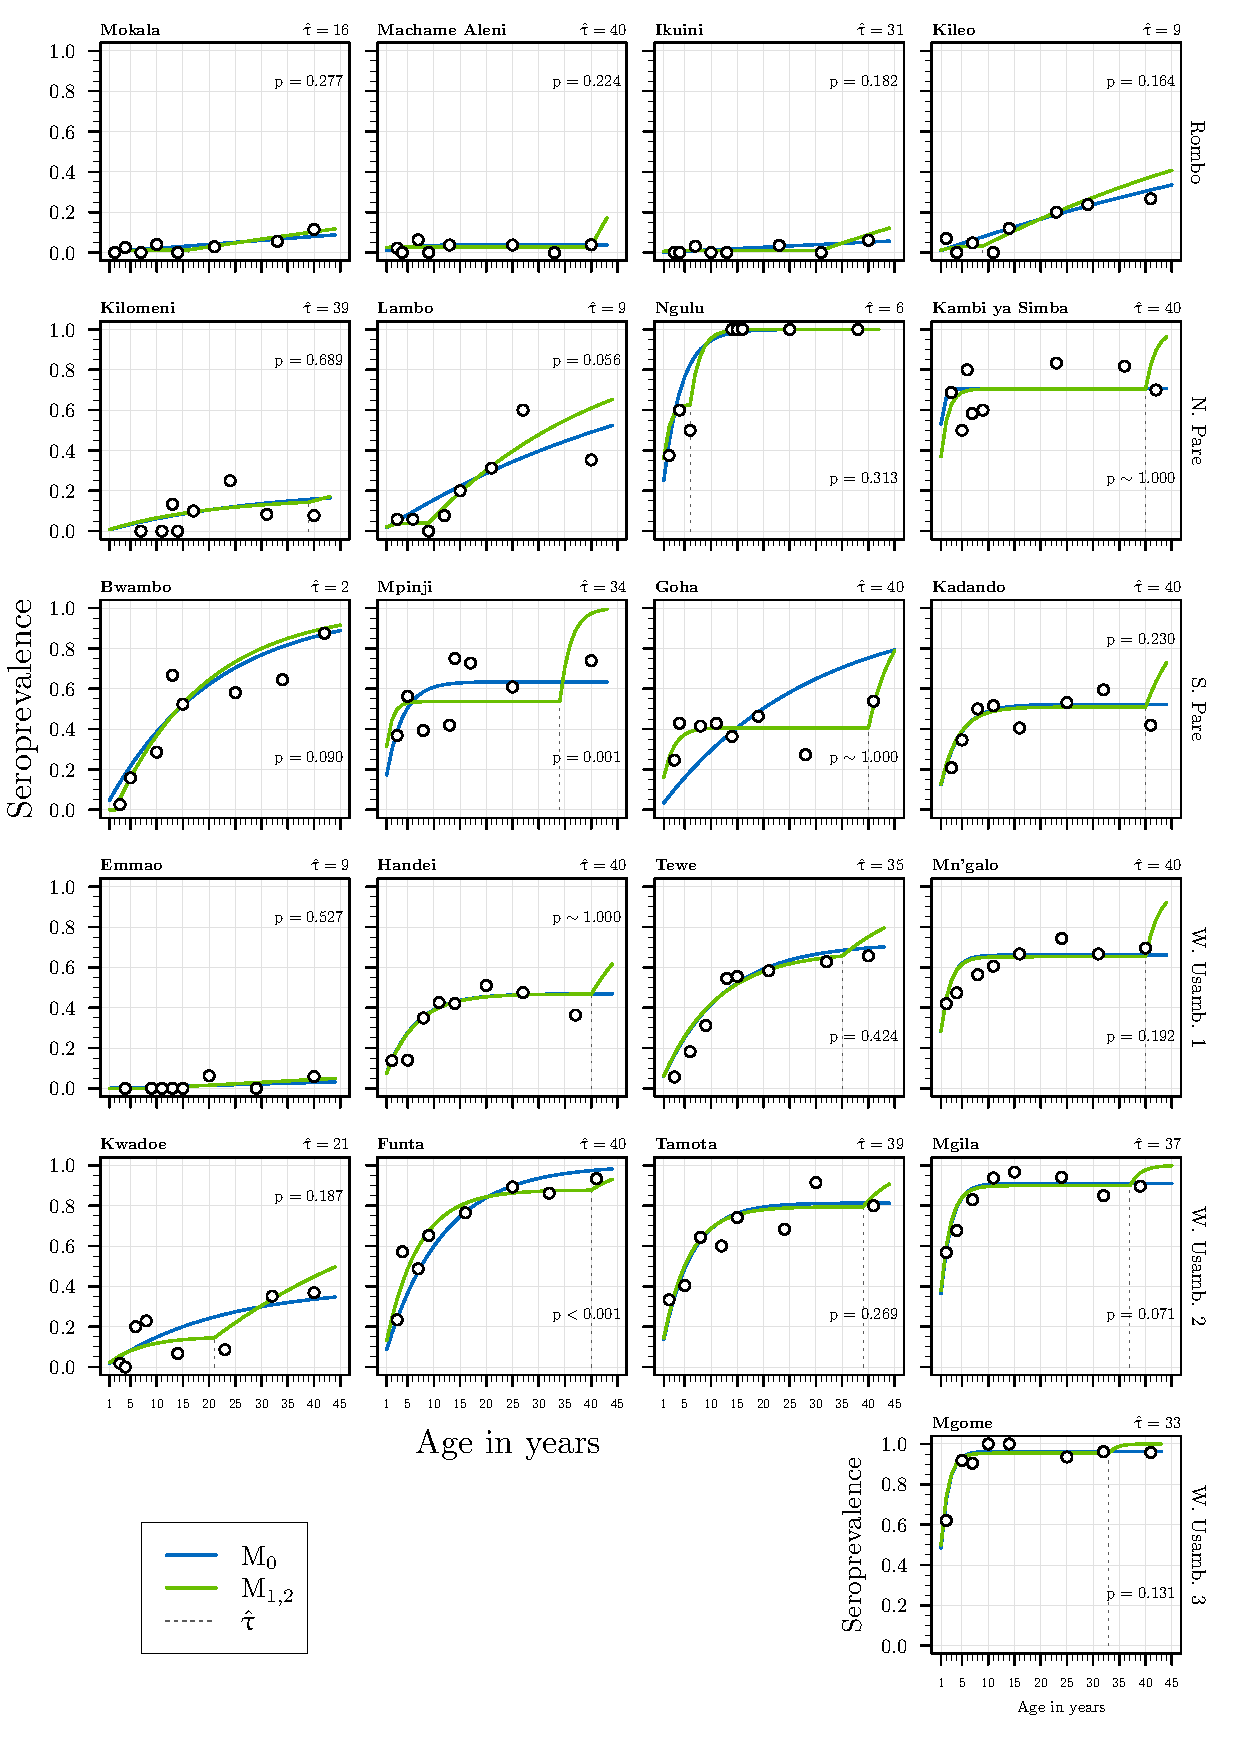
\includegraphics[width=\columnwidth]{images/Seroprevalence_M0vM12_msp2.pdf}
\end{adjustbox}
\caption[Estimated MSP2 seroprevalence for models M$_0$ and M$_{1,2}$]{Fits for the estimated MSP2 antigen seroprevalence for the 21 assessed villages, using models M$_0$ (blue lines) and M$_{1,2}$ (green lines), with the cutoff parameter of the latter signalled. Each row of graphs represents data from the transects (identified on the right hand side), where villages are ordered by decreasing altitude (and increasing malaria incidence). In the different plots, the dots represent the observed seroprevalence of distinct age groups by splitting the sampled age distribution into similar bins. P-values from the resulting likelihood ratio tests are identified.}
\label{fig:msp2.seroprevalence.M0.M12}
\end{figure}


\begin{figure}[H]
\center
\begin{adjustbox}{width=\linewidth,totalheight=\textheight-5\baselineskip}
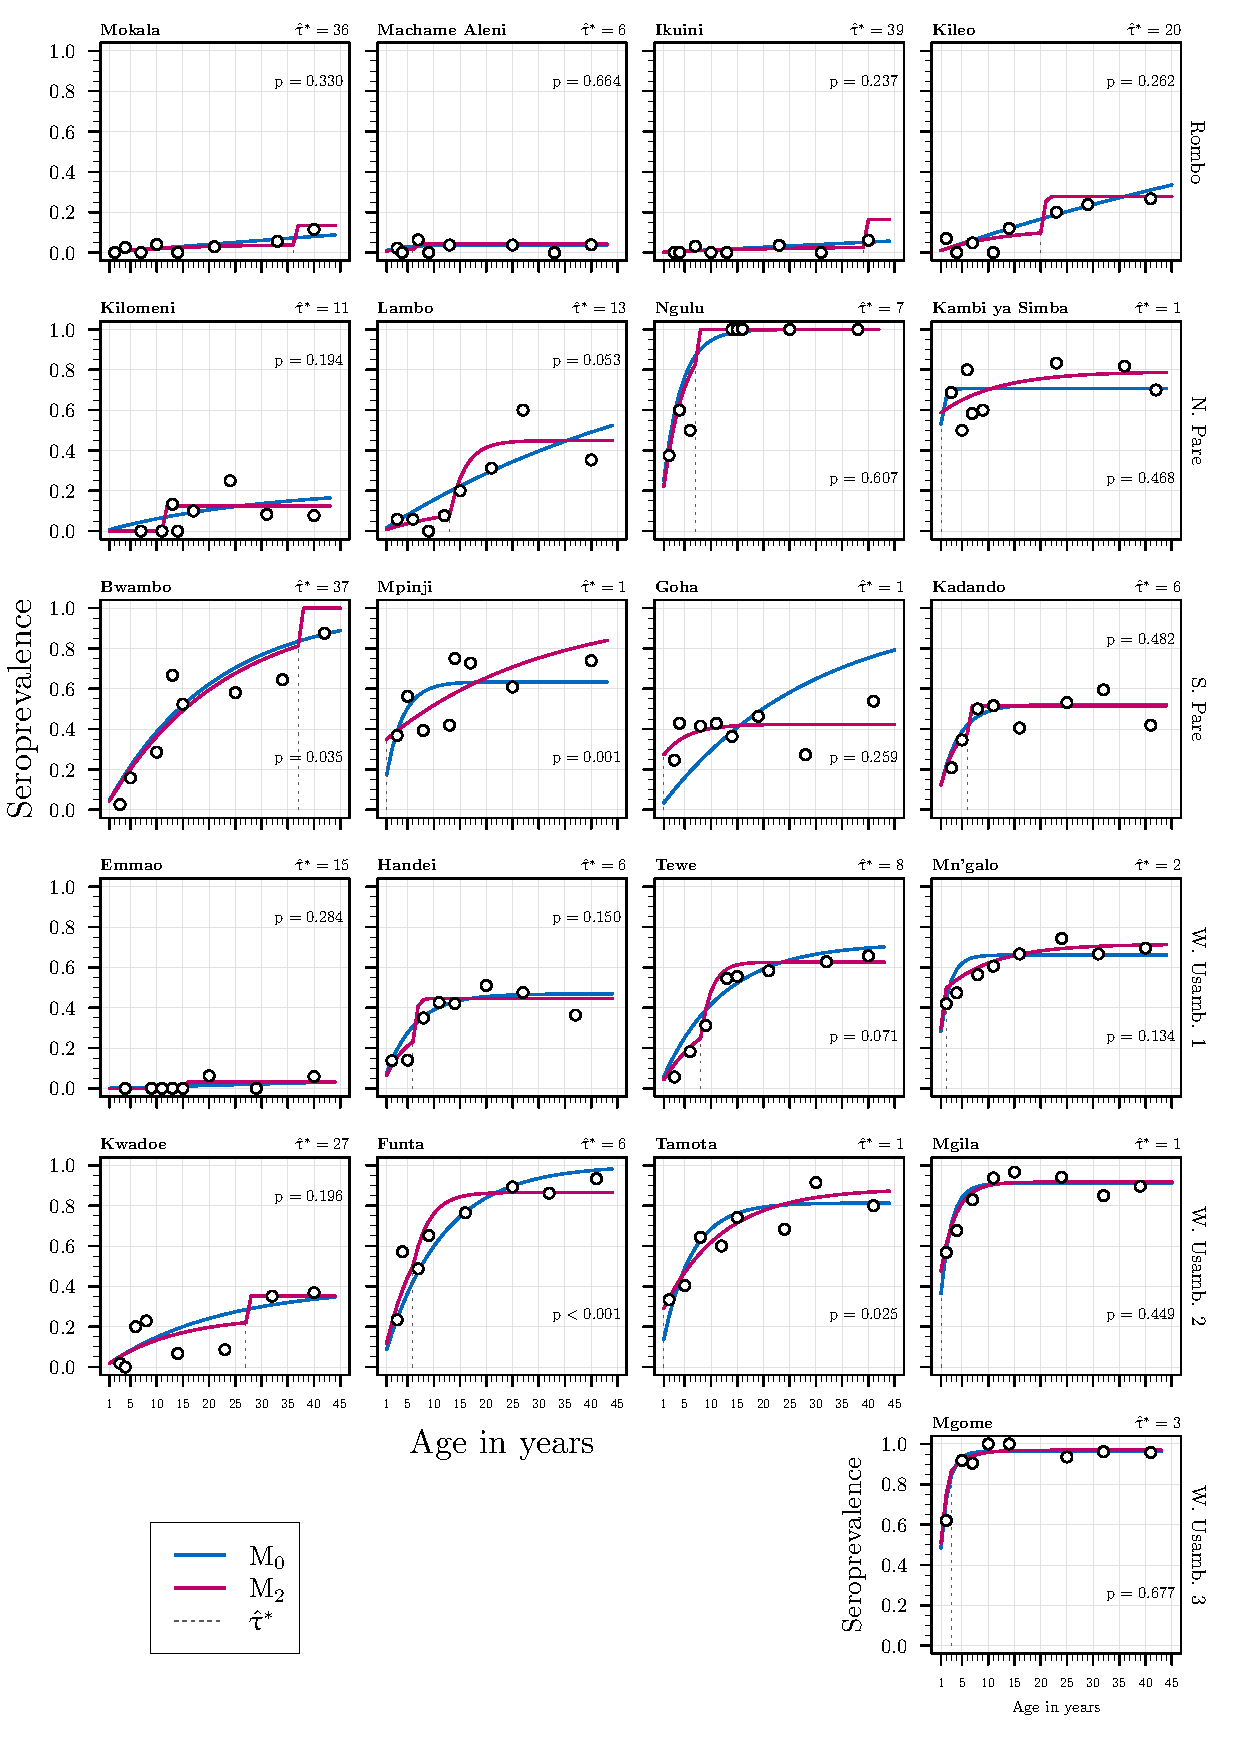
\includegraphics[width=\columnwidth]{images/Seroprevalence_M0vM2_msp2.pdf}
\end{adjustbox}
\caption[Estimated MSP2 seroprevalence for models M$_0$ and M$_2$]{Fits for the estimated MSP2 antigen seroprevalence for the 21 assessed villages, using models M$_0$ (blue lines) and M$_2$ (light red lines), with the cutoff parameter of the latter signalled, identifying the change in SCR happening in years before sampling. Each row of graphs represents data from the transects (identified on the right hand side), where villages are ordered by decreasing altitude (and increasing malaria incidence). In the different plots, the dots represent the observed seroprevalence of distinct age groups by splitting the sampled age distribution into similar bins. P-values from the resulting likelihood ratio tests are identified.}
\label{fig:msp2.seroprevalence.M0.M2}
\end{figure}

%%%%%%%%%%%%%%%%%%%%%%%%%%%%%%%%%%%%%%%%%%%%%%
% MODEL M2 ESTIMATED SEROPREVALENCE FOR AMA1 %
%%%%%%%%%%%%%%%%%%%%%%%%%%%%%%%%%%%%%%%%%%%%%%
\subsection{AMA1 estimated seroprevalence} \label{appendix:M2.seroprev.ama1}

\begin{figure}[H]
\center
\begin{adjustbox}{width=\linewidth,totalheight=\textheight-6\baselineskip}
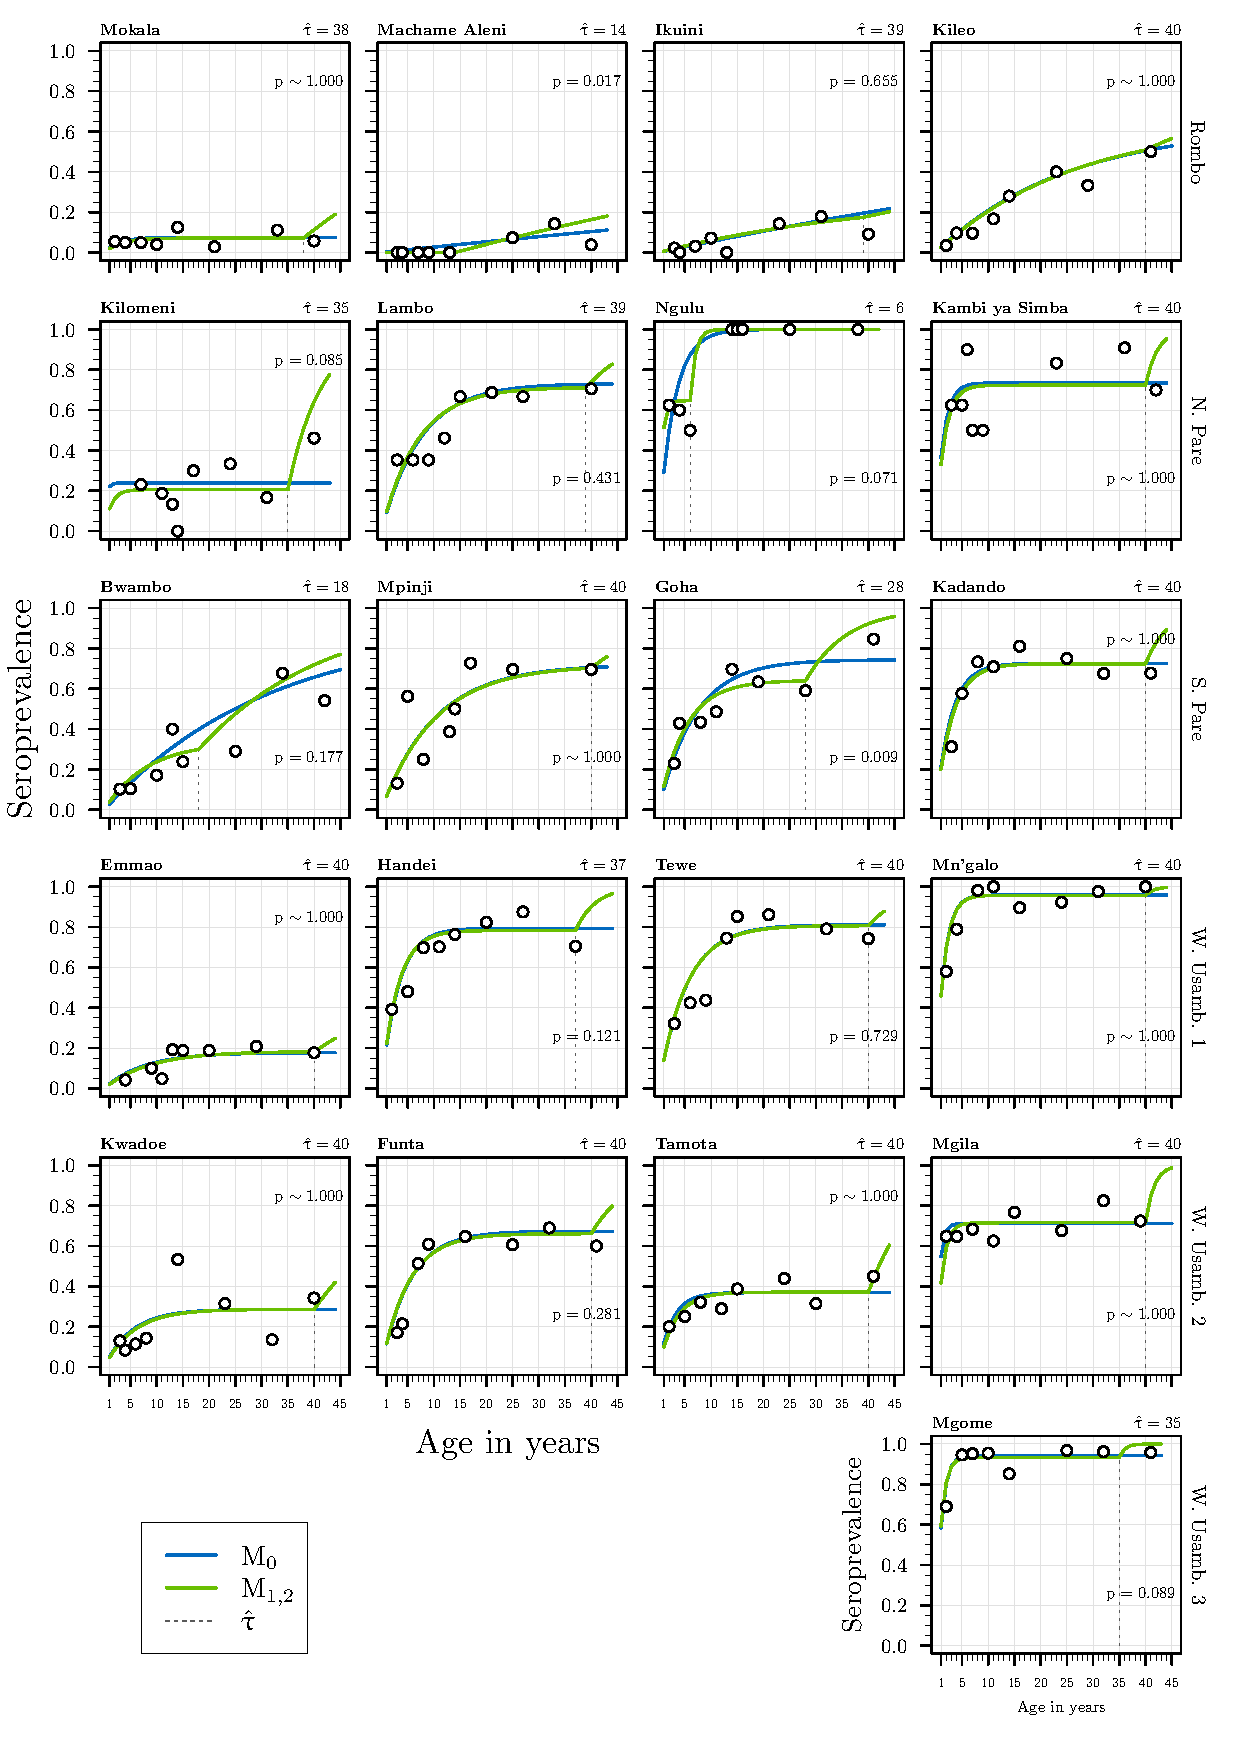
\includegraphics[width=\columnwidth]{images/Seroprevalence_M0vM12_ama1.pdf}
\end{adjustbox}
\caption[Estimated AMA1 seroprevalence for models M$_0$ and M$_{1,2}$]{Fits for the estimated AMA1 antigen seroprevalence for the 21 assessed villages, using models M$_0$ (blue lines) and M$_{1,2}$ (green lines), with the cutoff parameter of the latter signalled. Each row of graphs represents data from the transects (identified on the right hand side), where villages are ordered by decreasing altitude (and increasing malaria incidence). In the different plots, the dots represent the observed seroprevalence of distinct age groups by splitting the sampled age distribution into similar bins. P-values from the resulting likelihood ratio tests are identified.}
\label{fig:ama1.seroprevalence.M0.M12}
\end{figure}

\begin{figure}[H]
\center
\begin{adjustbox}{width=\linewidth,totalheight=\textheight-5\baselineskip}
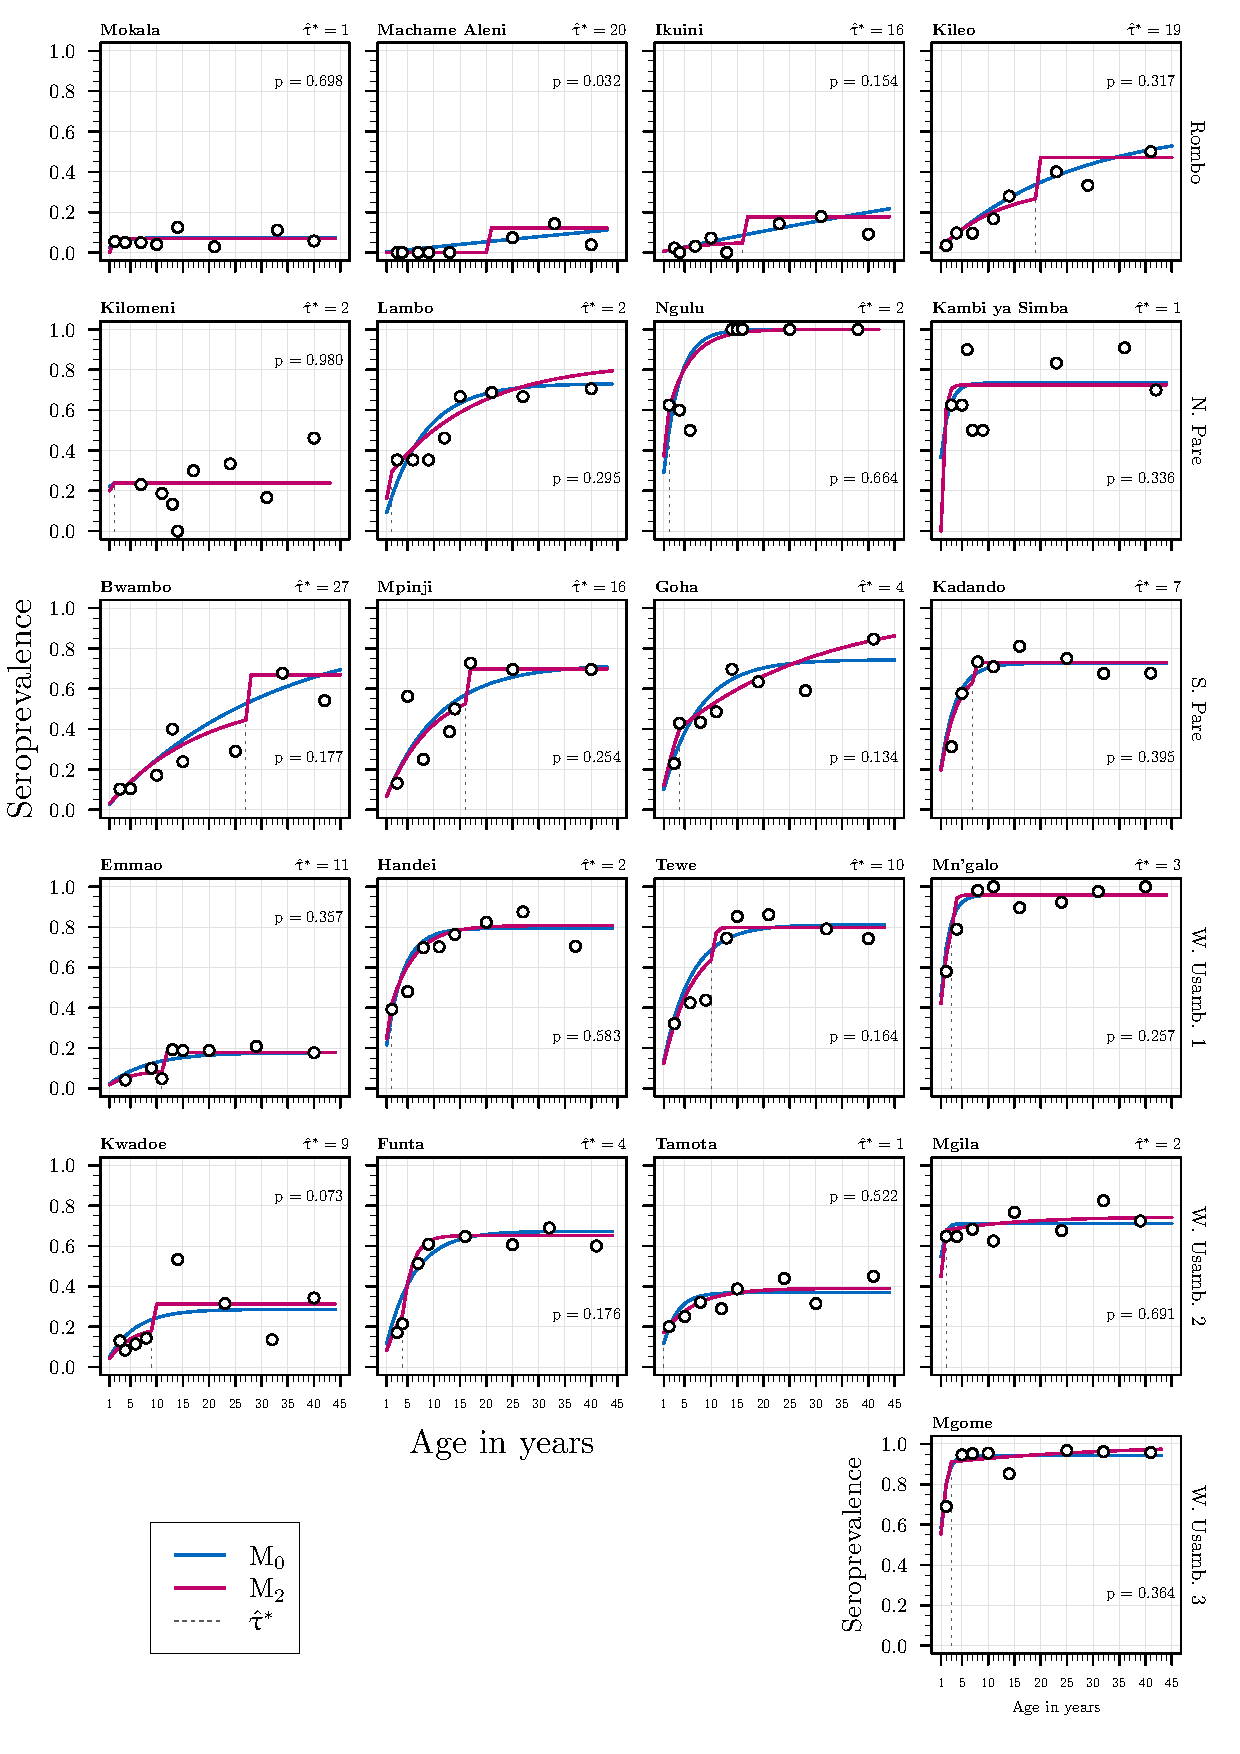
\includegraphics[width=\columnwidth]{images/Seroprevalence_M0vM2_ama1.pdf}
\end{adjustbox}
\caption[Estimated AMA1 seroprevalence for models M$_0$ and M$_2$]{Fits for the estimated AMA1 antigen seroprevalence for the 21 assessed villages, using models M$_0$ (blue lines) and M$_2$ (light red lines), with the cutoff parameter of the latter signalled, identifying the change in SCR happening in years before sampling. Each row of graphs represents data from the transects (identified on the right hand side), where villages are ordered by decreasing altitude (and increasing malaria incidence). In the different plots, the dots represent the observed seroprevalence of distinct age groups by splitting the sampled age distribution into similar bins. P-values from the resulting likelihood ratio tests are identified.}
\label{fig:ama1.seroprevalence.M0.M2}
\end{figure}



%%%%%%%%%%%%%%%%%%%%%%%%%%%%%%%%%%%%%%%%%%%%%%%%%%%%%
% R FUNCTIONS TO ESTIMATE TRANSITION RATES FROM M11 %
%%%%%%%%%%%%%%%%%%%%%%%%%%%%%%%%%%%%%%%%%%%%%%%%%%%%%

\subsection{R functions used to estimate transition rates from model M$_{1,1}$}
\label{appendix:r.function}
\definecolor{mygreen}{rgb}{0,0.6,0}
\definecolor{mygray}{rgb}{0.5,0.5,0.5}
\definecolor{mymauve}{rgb}{0.58,0,0.82}
\lstset{
        language=R,
        basicstyle=\scriptsize\ttfamily,
        commentstyle=\ttfamily\color{mygreen},
        numbers=left,
        numberstyle=\ttfamily\color{black}\footnotesize,
        stepnumber=1,
        numbersep=5pt,
        backgroundcolor=\color{white},
        showspaces=false,
        showstringspaces=false,
        showtabs=false,
        frame=single,
        tabsize=2,
        captionpos=b, % sets the caption-position to bottom
        breaklines=true, % sets automatic line breaking
        breakatwhitespace=false, % sets if automatic breaks should only happen at whitespace
        title=\lstname,
        escapeinside={},
        keywordstyle={},
        morekeywords={},
        backgroundcolor=\color{white}, % choose the background color; you must add \usepackage{color} or \usepackage{xcolor}; should come as last argument
        keepspaces=true,                 % keeps spaces in text, useful for keeping indentation of code (possibly needs columns=flexible)
        keywordstyle=\ttfamily\color{blue},       % keyword style
        morekeywords={*,...},            % if you want to add more keywords to the set
        numbersep=5pt,                   % how far the line-numbers are from the code
        rulecolor=\color{black},         % if not set, the frame-color may be changed on line-breaks within not-black text (e.g. comments (green here))
        title=\ttfamily{jtm\_functions\_M11.R}
}

\lstinputlisting[language=R]{appendices/jtm_functions_M11.R}

\end{appendices}